\documentclass[a4paper,12pt]{scrartcl}
\usepackage{setspace}
\usepackage[utf8x]{inputenc}
\usepackage{ngerman}
\usepackage{graphicx}
\usepackage{enumerate}
\usepackage{float}
\usepackage[font=small,labelfont=bf,singlelinecheck=false]{caption}
\usepackage[headsepline,plainheadsepline]{scrpage2}
\pagestyle{scrheadings}
\ohead[]{Christian Casar, Maximilian Menzel}
\ihead{HR - Blatt 5}



\begin{document}
\parindent0mm
\restylefloat{figure}
\setcapindent{0pt}
\subsubsection*{Parallelisierung mit Pthreads}
Wie Tabelle 1 zu entnehmen haben wir mit unserer Parallelisierung durch Pthreads eine Leistungssteigerung um den Faktor 9,8 bei der Verwendung von 12 Threads gegenüber dem sequentiellen Programm erreicht. Die Abnahme der Messwerte für zunehmende Threadanzahl entspricht dem erwartetem Umfang: Bei einer Verdoppelung der Threads erreichen wir eine Halbierung der Laufzeit.
\begin{table}[!ht]
\begin{tabular}{|l|r|r|}
\hline
\#Threads&Mittelwert&Varianz \\
\hline
sequentiell&1147.1261 &0.1684\\
\hline
01 &1144.5818 &   0.3273 \\ 
\hline
02 &604.3500   & 0.2344  \\
\hline
03      &    429.3624   & 59.9607  \\
\hline 
04         & 325.1812  &   3.3782   \\
\hline
05       &  259.3620  &  0.0231  \\
\hline
06     &    217.6925  &  0.9406  \\
\hline
07     &     185.5498   &  0.0013  \\      
\hline
08     &    162.9680  &  0.6020  \\
\hline
09     &     146.7405 &   0.8329  \\
\hline
10     &   133.1081   &  2.1805  \\ 
\hline
11     &    125.0790  &   7.0599  \\  
\hline
12    &  117.5398  &   7.2995\\
\hline
\end{tabular}
\caption{\textbf{Zeitmessung mit variierender Threadzahl.}\\ 512 Interlines, 1024 Iterationen, 5 Messungen, Messwerte in\\ Sekunden }
\end{table}

\begin{figure}[H]
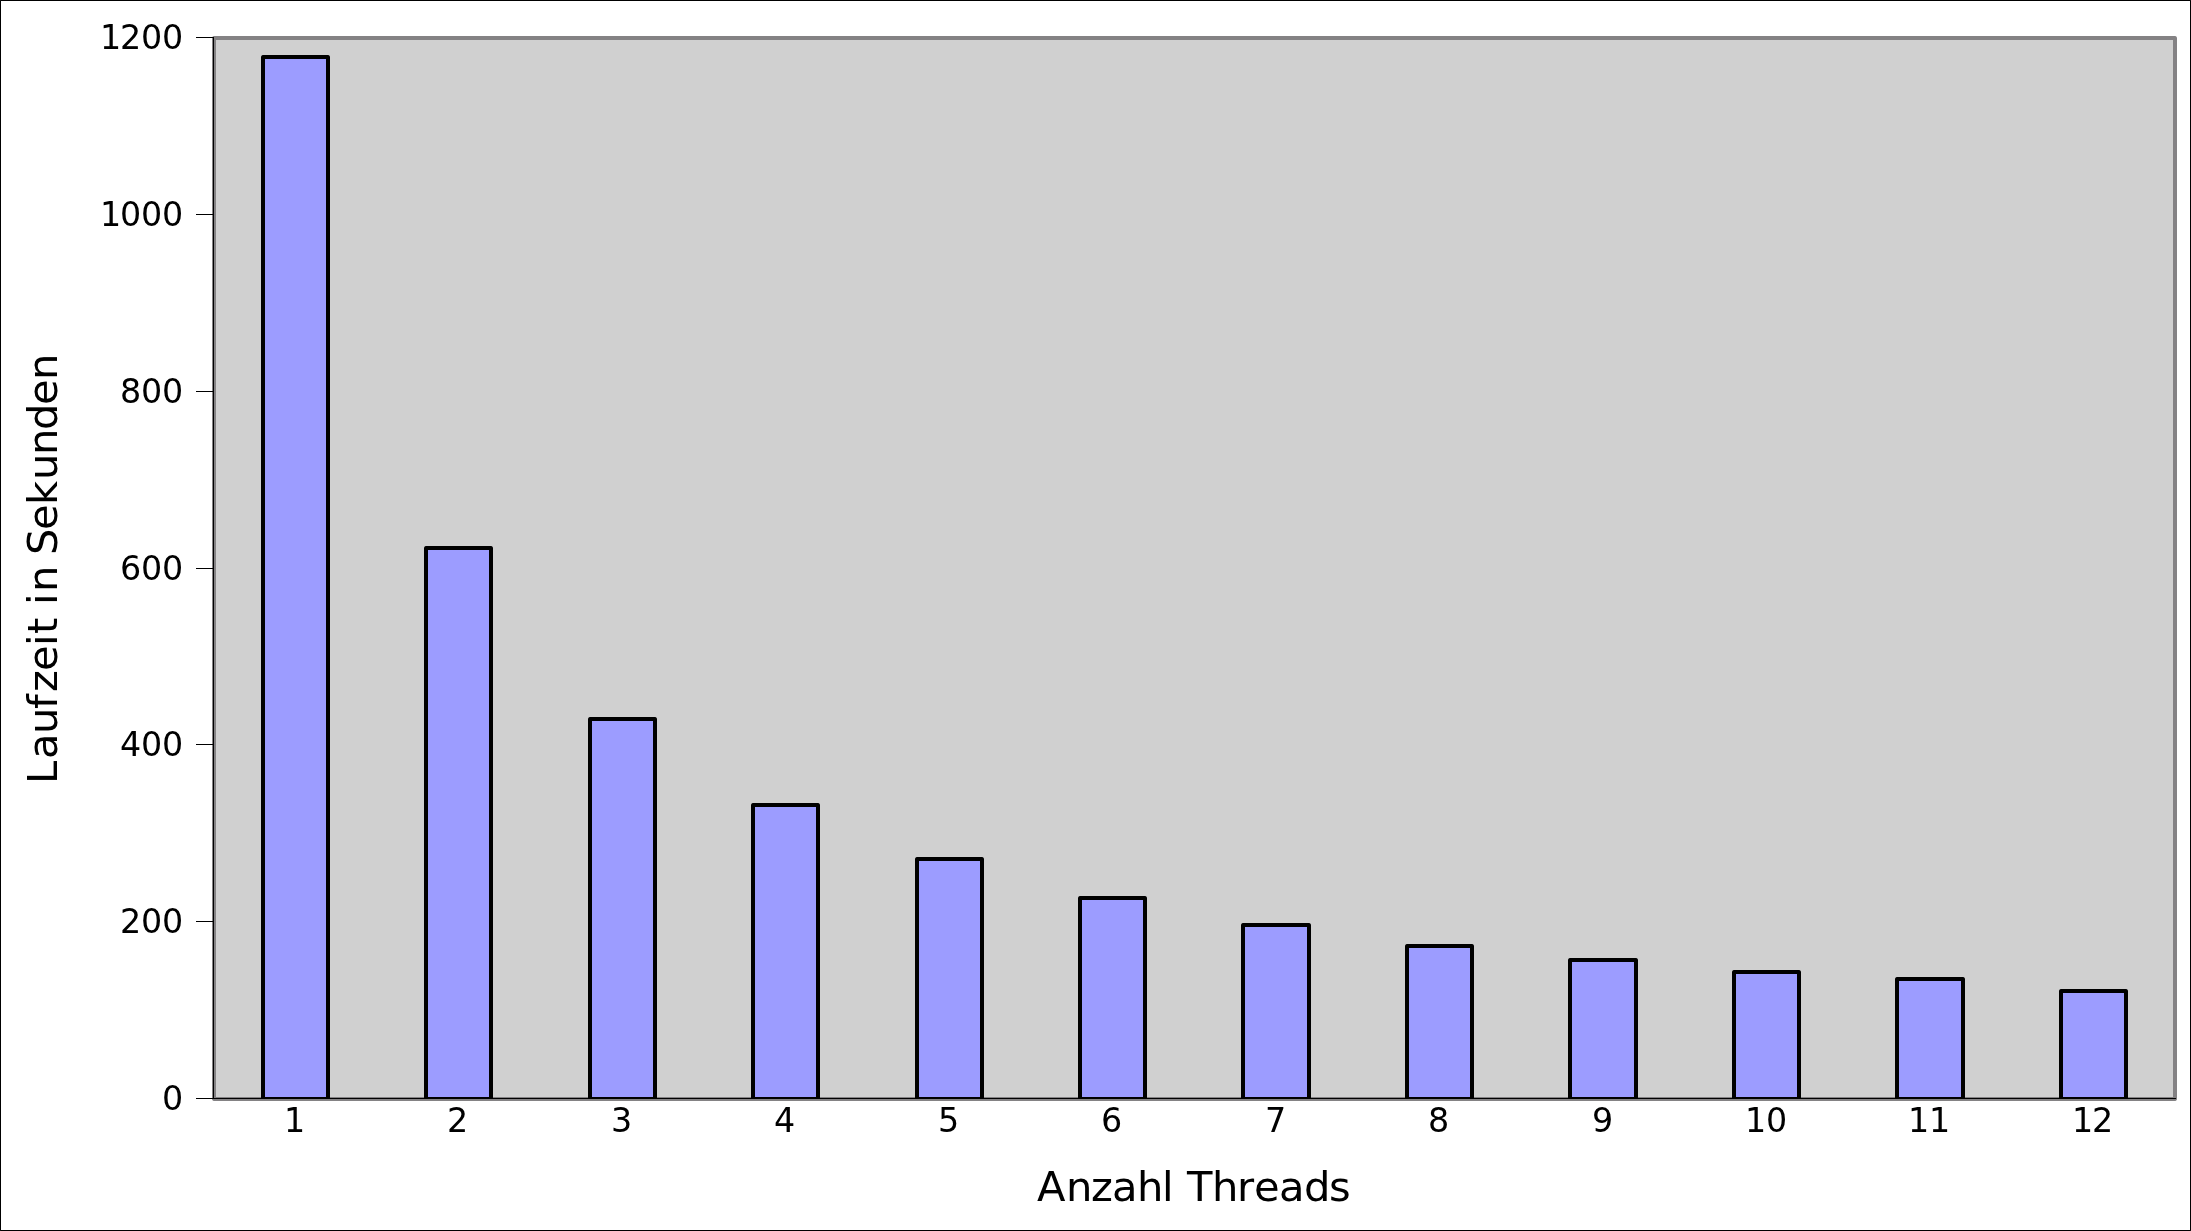
\includegraphics[width=13cm]{/home/christian/Uni/5_Semester/HR/HR-1213/Blatt5/leistungsgraph.png}
\caption{\textbf{Laufzeitmessung für verschiedene Threadzahlen.} 12 Threads,\\ 1024 Iterationen, Messwerte jeweils in Sekunden}
\end{figure}
\end{document}
